\scanpage{82}
% archive foliation: 81
\uline{écart additif}
\[
A_1(f,g)=dg/df=\frac{g'}{f'}
\qquad A_n(f,g)=\left(\frac{dg}{df}\right)^n
=\left(\frac{g'}{f'}\right)^n
\]
\deleted{\unsure{écart}}

\uline{écart affine}
\[
\operatorname{Aff}(f,g)=D_{dg}-D_{df}
=\frac{d\,\dfrac{dg}{df}}{dg/df}
=\frac{d\,\dfrac{g'}{f'}}{g'/f'}
=\frac{dg'}{g'}-\frac{df'}{f'}
=\left(\frac{g''}{g'}-\frac{f''}{f'}\right)dt
\]
\diagram{\begin{tikzcd}[column sep=small,row sep=large]
& &\substack{E_X/(\mu_n.G_a)(\mathbf C)
\overset{\sim}{\longrightarrow}\underline\omega_X^n\\
c_{a,n}(f)=(df)^n\\\text{torseur sous }\underline O_X^*}
\arrow[r,"{(n=0)}"]
&\substack{E_X/(G_m.G_a)(\mathbf C)
\overset{\sim}{\longrightarrow}\operatorname{Conn}(\underline\omega_X^1)\\
c_{af}(f)=D_{df}\\\text{torseur sous }\underline\omega_X^1}
\arrow[d,"{D\mapsto c_D}"]\\
E_X\arrow[r]\arrow[dd,dashed,"\exp"']
&\substack{E_X/G_a(\mathbf C)\overset{\sim}{\longrightarrow}
\underline\omega_X^{1*}\\c_a(\deleted{\unsure{f}}f)=df\\
\text{torseur sous }\underline O_X^*}
\arrow[ur]\arrow[dd,bend right=14,"?"']\arrow[dd,bend left=14,"\mathrm{id}"]
&&\substack{P_X/GP(1,\mathbf C)\overset{\sim}{\longrightarrow}
\operatorname{Conn\,proj}(X)\\c_{pr}(f)=c_{D_{df}}\\
\underline\omega_X^2\quad(\text{torseur sous})}\\
&&\substack{E_X^*/(\mathbf Z/2\mathbf Z.G_m)(\mathbf C)
\simeq\underline\omega_X^{2*}\\\text{torseur sous }\underline O_X^*}&\\
E_X^*\arrow[r]
&\substack{E_X^*/G_m(\mathbf C)\overset{\sim}{\longrightarrow}
\underline\omega_X^{1*}\\c_m(f)=df/f\\
\text{torseur sous }\underline O_X^*}\arrow[ur]&&
\end{tikzcd}}
\margin{$\unsure{r|f}$;\quad\deleted{$\unsure{E_X^*}$};\quad
\deleted{$E_X\unsure{?}$};\quad $E_X$}
\[
\underline O_X^*\xrightarrow{\varphi\mapsto\varphi^n}\underline O_X^*
\xrightarrow{\varphi\mapsto-\frac1n\frac{d\varphi}{\varphi}}
\underline\omega_X^1
\qquad
\underline O_X^*\xrightarrow{\varphi\mapsto\varphi^2}\underline O_X^*
\]
\[
\boxed{c_{D+\omega_1}=c_D+2D\omega_1+\omega_1^2}
\]
\figure{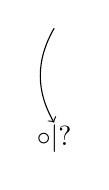
\begin{tikzpicture}[x=1cm,y=1cm]
\draw[->] (0,1.2) to[bend right=30] (0,0);
\node at (0,-.2) {$\unsure{\circ|?}$};
\end{tikzpicture}}
\[
\exp(\pm f+a)=\underline{\unsure{\exp a|e^a}}(\exp f)^{\pm1}
\]
\figure{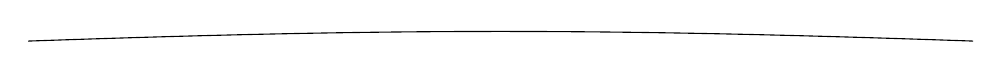
\begin{tikzpicture}\draw (0,0) to[bend left=2] (12,0);\end{tikzpicture}}

\[
\operatorname{Ecad}(f,g)=\frac{dg}{df}=\frac{g'}{f'}\in\Gamma\underline O_X^*
\]
\[
\unsure{\operatorname{Ecaf}_n|\operatorname{Ecad}_n}(f,g)
=\left(\frac{dg}{df}\right)^n=\left(\frac{g'}{f'}\right)^n
\in\Gamma(\underline O_X^*)
\]
\[
\operatorname{Ecaf}(f,g)=\frac{d(dg/df)}{dg/df}
=\frac{d(g'/f')}{g'/f'}=\frac{dg'}{g'}-\frac{df'}{f'}
=\left(\frac{g''}{g'}-\frac{f''}{f'}\right)dt
\in\Gamma(\underline\omega_X^1)
\]
\[
\operatorname{Ecmu}_1(f,g)=\frac{dg/g}{df/f}
=\frac{g'/g}{f'/f}\in\Gamma(\underline O_X^*)
\]
\[
\operatorname{Ecmu}_2(f,g)=\left(\frac{dg/g}{df/f}\right)^2
=\left(\frac{g'/g}{f'/f}\right)^2\in\Gamma(\underline O_X^*)
\]
\[
\begin{aligned}
\operatorname{Ecpr}(f,g)
&=-2\frac{d^3g/df^3}{dg/df}+3\left(\frac{d^2g/df^2}{dg/df}\right)^2\\
&=\left[\left(-2\frac{g'''}{g'}+3\left(\frac{g''}{g'}\right)^2\right)
-\left(-2\frac{f'''}{f'}+3\left(\frac{f''}{f'}\right)^2\right)\right]dt^2
\in\Gamma(\underline\omega_X^{\unsure{1|2}})
\end{aligned}
\]

\diagram{\begin{tikzcd}[column sep=small,row sep=large]
E_X\arrow[r,"d"]\arrow[ddd,"\exp"']
&\left[\substack{E_X/G_a(\mathbf C)\overset{\sim}{\longrightarrow}
\underline\omega_X^{1*}\\c_a(f)=df}\right]
\arrow[r,"\alpha_n"]\arrow[ddd,bend right=12,"?"']
\arrow[ddd,bend left=12,"\mathrm{id}"]
&\left[\substack{E_X/(\mu_n.G_a)(\mathbf C)
\overset{\sim}{\longrightarrow}\underline\omega_X^{n*}\\c_{a,n}(f)=(df)^n}\right]
\arrow[r,"\beta_n"]\arrow[ddd,"{\mathrm{id}\ (n=2)}"]
&\left[\substack{E_X/(G_m.G_a)(\mathbf C)\simeq
\operatorname{Conn}(\underline\omega_X)\\c_{af}(f)=D_{df}}\right]
\arrow[dd,"\gamma"]\\
&\underline O_X^*\arrow[r,"{\varphi\mapsto\varphi^n}"]\arrow[d,"\mathrm{id}"']
&\underline O_X^*\deleted{\unsure{\underline O_X^*}}
\arrow[r,"{\varphi\mapsto-\frac1n\frac{d\varphi}{\varphi}}"]
\arrow[d,"\mathrm{id}"']&\underline\omega_X\\
&\underline O_X^*\arrow[r,"{\varphi\mapsto\varphi^2}"']
&\underline O_X^*\arrow[r,bend right=15]
&\substack{[P_X/GP(1,\mathbf C)\simeq\operatorname{Conn}(X)]\\
\underline\omega_X^2}\\
E_X^*\arrow[r]
&\left[\substack{E_X^*/G_m(\mathbf C)\simeq\underline\omega_X^{1*}\\
c_m(f)=df/f}\right]\arrow[r,"{\alpha'_2}"]
&[E_X^*/(\mathbf Z/2\mathbf Z.G_m)(\mathbf C)\simeq\underline\omega_X^{2*}]
\arrow[ur,bend right=15,"\delta"']&
\end{tikzcd}}

\[
\alpha_n(\omega_1)=\omega_1^n
\]
\[
\begin{aligned}
\beta_n(\omega_n)&=\beta_1(\omega_n^{1/n})
=\beta_1(f^{1/n}dt)\\
&=D_{dt}\deleted{\unsure{\omega_1}}
+\unsure{-\frac1n|\frac1n}\frac{df}{f}
=D_{dt}+\unsure{-\frac1n|\frac1n}\frac{f'}f\,dt
\end{aligned}
\]
\margin{$\unsure{\beta_1(fdt)}$}
\[
\begin{aligned}
\gamma(D_{dt}+\underset{\Vert\ fdt}{\omega_1})
&=\underset{\Vert\ c_{pr}(t)}{\gamma(D_{dt})}
+2D_{dt}\omega_1+\omega_1^2\\
&=c_{pr}(t)+2\frac{df}{\unsure{dt}}dt+f^2dt^2
=c_{pr}(t)+(2f'+f^2)dt^2
\end{aligned}
\]
\[
\begin{aligned}
\gamma\beta_n(\omega_n)
&=c_{pr}(t)+\left(2\left(-\frac1n\frac{f'}f\right)'
+\left(-\frac1n\frac{f'}f\right)^2\right)dt^2\\
&=c_{pr}(t)+\frac1{n^{\unsure{2}}}
\left(-2n\frac{f''}f+\inserted{\unsure{(2n+1)}}
\deleted{\unsure{1}}\left(\frac{f'}f\right)^2\right)dt^2\\
&=c_{pr}(t)+\left(-2\frac{f''}f+3\left(\frac{f'}f\right)^2\right)dt^2
\end{aligned}
\]
\margin{$\gamma\beta_1(\omega_1)$}
\[
\gamma\beta_1d(f)=c_{pr}(t)+\deleted{\unsure{\frac1{n^2}}}
\left(-2\frac{f'''}{f'}+3\left(\frac{f''}{f'}\right)^2\right)dt^2
\]
\margin{\[
\begin{aligned}
\delta(\omega_2)&=\gamma\beta_2(\omega_2)+\omega_2\\
&=c_{pr}(\unsure{t|\omega_1})+
\left[f-\unsure{\frac{f''}f|2\frac{f''}f}+\frac54\left(\frac{f'}f\right)^2\right]dt^2\\
\delta\alpha'_2(\omega_1)&=\gamma\beta_1(\omega_1)
\deleted{\unsure{^{2}}}+\omega_1^{\unsure{2|1}}\\
&=c_{pr}(t)+\left[f^2-2\frac{f''}f+3\left(\frac{f'}f\right)^2\right]dt^2
\end{aligned}
\]}
\figure{\begin{tikzpicture}[x=1cm,y=1cm]
\draw (0,2) to[bend left=3] (0,0) to[bend right=3] (3,0);
\draw (.1,2)--(.1,.3);
\end{tikzpicture}}

